\subsection{UC9 - Salvataggio visualizzazione}
    \label{uc9}
    \begin{figure}[htbp]
        \centering
        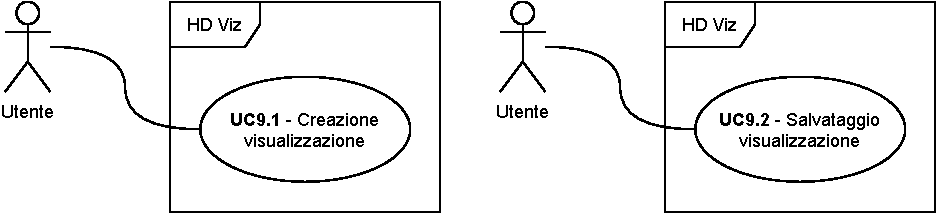
\includegraphics[width=0.45\textwidth]{source/sections/casi-uso/diagrams/uc9.pdf}
        \caption{UC9 - Salvataggio visualizzazione}
        \label{fig:uc9}
    \end{figure}
    \begin{itemize}
    \item \textbf{Attore}: utente;
    \item \textbf{Descrizione}: l'utente salva la visualizzazione;
    \item \textbf{Precondizione}: 
    \begin{itemize}
        \item eseguito l'upload del dataset come matrice $N\times M$ (\hyperref[uc1]{UC1});
        \item eseguito un tipo di visualizzazione (\hyperref[uc2]{UC2});
    \end{itemize}  
    \item \textbf{Postcondizione}: l'utente ha salvato la visualizzazione come file immagine PNG;
    \item \textbf{Output}: file PNG con la visualizzazione richiesta;
    \item \textbf{Scenario Principale}: 
    \begin{enumerate}
        \item l'utente carica il suo dataset (\hyperref[uc1]{UC1});
        \item l'utente visualizza il dataset tramite un grafico tra quelli resi disponibili (\hyperref[uc2]{UC2});
        \item l'utente salva la visualizzazione in formato PNG.
    \end{enumerate}
    \end{itemize}